\documentclass[11pt]{amsbook}

\usepackage{../HBSuerDemir}	% ------------------------


\begin{document}

% ++++++++++++++++++++++++++++++++++++++
\hPage{b2p2/390}
% ++++++++++++++++++++++++++++++++++++++

% =======================================
    constant , the equations of \(PP_1\), \(PP_2\) will be 
    \[ g(x,y) = v , f(x,y) = u, \]
    so that along \(PP_1\), v remains constant while u varies, and along \(PP_2\), u remains constant while v varies. Therefore if P has coordinates F(u,v), G(u,v), those of the nearby points \(P_1\) and \(P_2\) will be
        \[ F(u + du, v), G(u + du, v); \]
        \[ F(u, v + dv), G(u, v + dv) \]
    and by the Mean Value Theorem, we have 
     \[ P(F(u, v), G(u, v)) \]
     \[ P_1(F(u, v) + F_u du, G(u, v) + G_u du) \]
     \[ P_2(F(u, v) + F_v dv, G(u, v) + G_v dv) \]

% =======================================
    \\ Now, since \(PP_1P_3P_2\) is nearly a paralelogram for small du, dv, the area dA is twice the area of the triangle \(PP_1P_2\):
    \[ dA = \left| PP_1P_2 \right| = \pm \left| \begin{array}{ccc}
        F & G & 1\\
        F + F_u du & G + G_u du & 1 \\
        F + F_v dv & G + G_v dv & 1 \end{array} \right|\]
    \[ = \pm \left| \begin{array}{ccc}
        F & G & 1\\
        F_u du & G_u du & 1 \\
        F_v dv & G_v dv & 1 \end{array} \right| = \pm \left| \begin{array}{cc}
        F_u & G_u\\
        F_v& G_v\\ \end{array} \right| \quad du \quad dv \]
        
    \[\Rightarrow dA = \pm \left| \begin{array}{cc}
        \frac{\partial F}{\partial u} & \frac{\partial G}{\partial u}\\[0.5em]
        \frac{\partial F}{\partial v} & \frac{\partial G}{\partial v}\\ \end{array} \right| \quad du \quad dv\]
    
    where + or - is taken to make the right hand side positive.
    
% =======================================================
    \\The determinant
    \[J = \left| \begin{array}{cc}
        \frac{\partial F}{\partial u} & \frac{\partial G}{\partial u}\\[0.5em]
        \frac{\partial F}{\partial v} & \frac{\partial G}{\partial v}\\ \end{array} \right| \quad or \quad J = \left| \begin{array}{cc}
        \frac{\partial x}{\partial u} & \frac{\partial y}{\partial v}\\[0.5em]
        \frac{\partial y}{\partial u} & \frac{\partial y}{\partial v}\\ \end{array} \right|\]
    is called the JACOBIAN of F, G (or of x, y) with respect to u, v, denoted by
    \[
        \frac{\partial (F, G)}{\partial (u,v)} \quad or \quad \frac{\partial (x, y)}{\partial (u,v)} \]
% =======================================

\end{document}  

%==== templates ====

%==== environments ====

%\begin{figure}[htb]
%	\centering
%	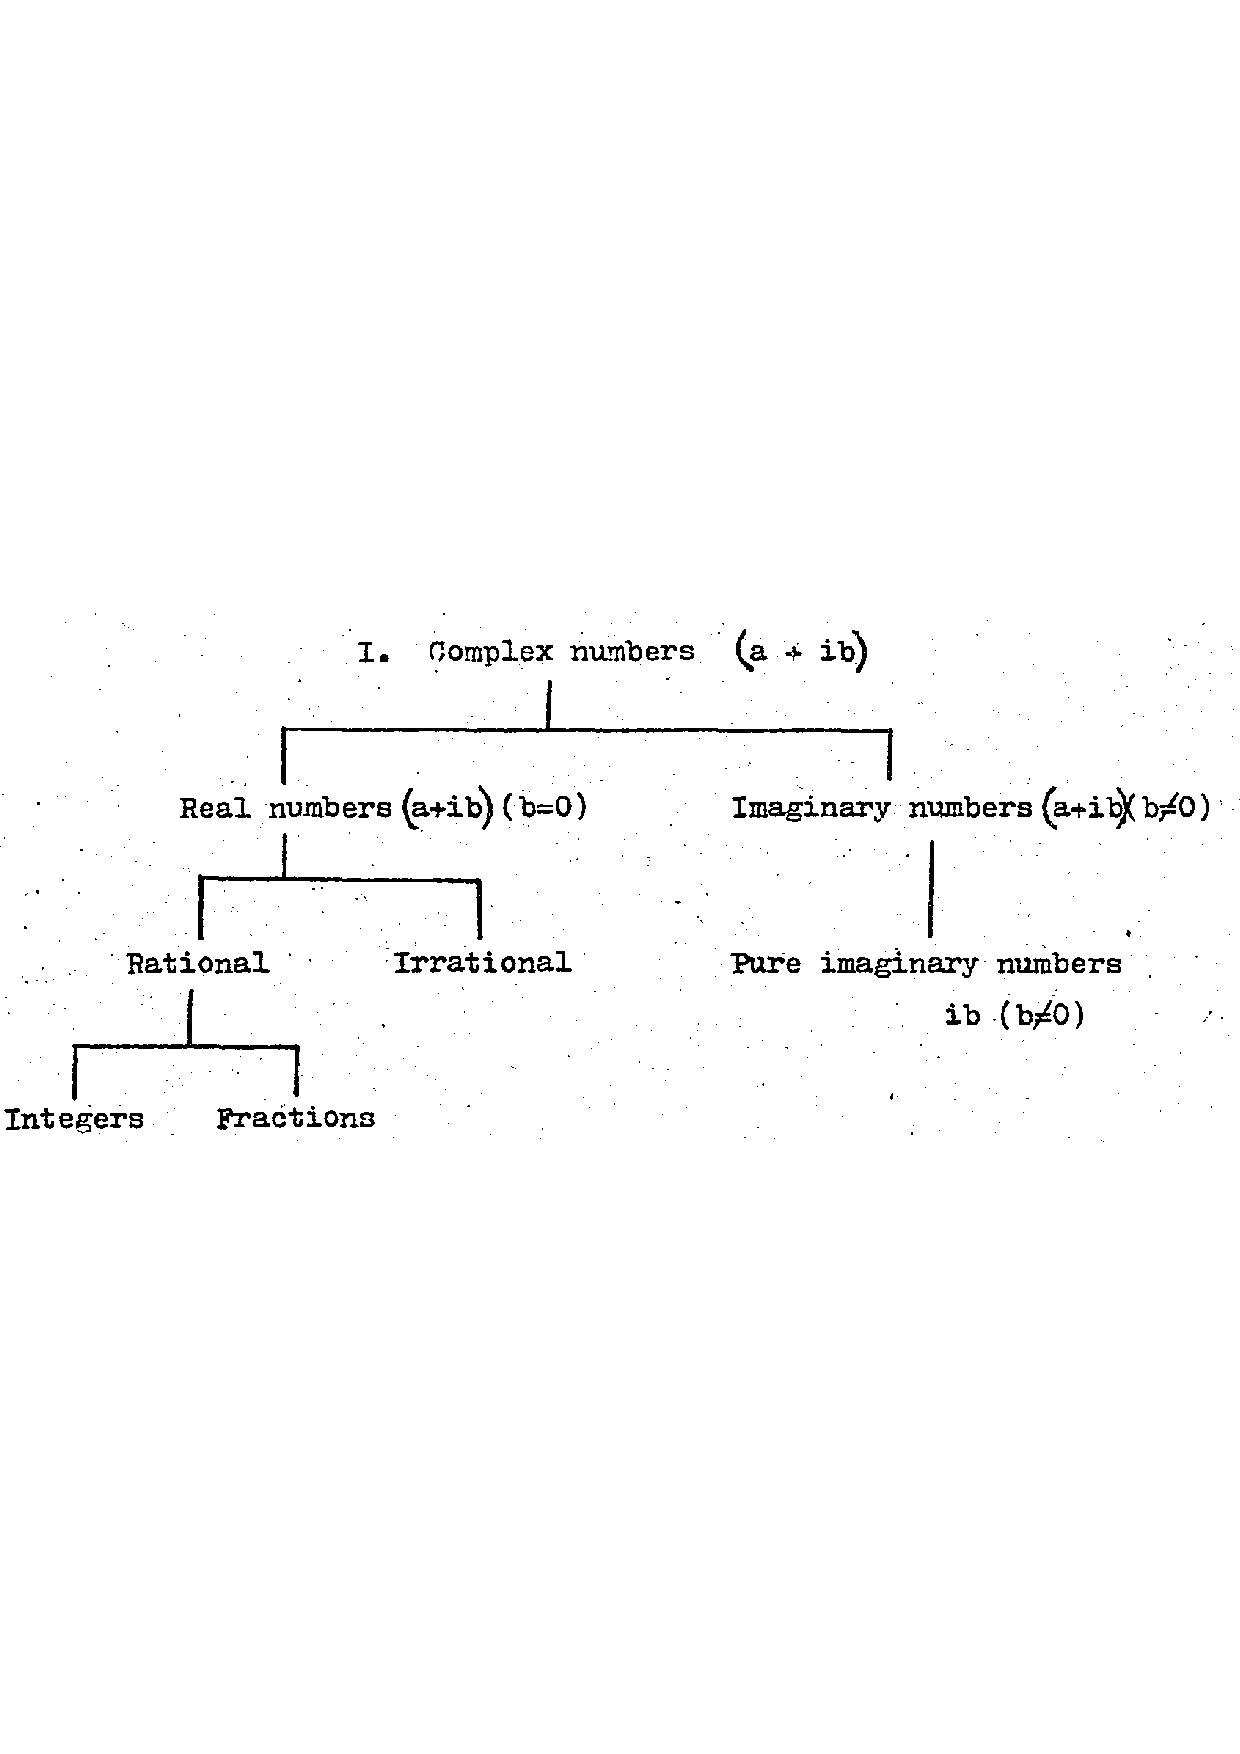
\includegraphics[width=0.9\textwidth]{images/SD-1-1p15A}
%	\caption{Classification of complex numbers}
%	\label{fig:classificationOfComplexNumbersA}
%\end{figure}

%\begin{center}
%\begin{tabular}{cc}
%\end{tabular}
%\end{center}

%\begin{exmp}
%\begin{hSolution}
%\end{hSolution}
%\end{exmp}

%\begin{hEnumerateAlpha}
%\end{hEnumerateAlpha}

%\begin{hEnumerateRoman}
%\end{hEnumerateRoman}

%$
%\begin{bmatrix}
%\end{bmatrix}
%$

%\frac{aaaa}{bbb}
%\frac{a_{n}}{b_{n}}
%\left( aaaa \right)
%\Longrightarrow

%\begin{multicols}{2}
%	bb
%\columnbreak
%	aa
%\end{multicols}